\chapter{Metastability of a Prefix Cache Under Load}\label{sec:L7}
% Generated by scripts/metastability_ctmc.py; do not edit.
\newcommand{\metaOpenTable}{\begin{tabular}{rrrr}\toprule
$\lambda$ (1/s) & $\lambda S^{\mathrm{miss}}$ & fluid saddle & mean time to collapse (s)\\\midrule
0.15 & 0.75 & -- & -- \\
0.19 & 0.95 & -- & -- \\
0.21 & 1.05 & 31 & $10^{16.2}$ \\
0.25 & 1.25 & 25 & $10^{13.9}$ \\
0.50 & 2.50 & 17 & $10^{7.5}$ \\
1.00 & 5.00 & 11 & $10^{3.2}$ \\
1.50 & 7.50 & 6 & $10^{1.9}$ \\
\bottomrule\end{tabular}}
\newcommand{\metaScalingTable}{\begin{tabular}{rrrrrr}\toprule
$N$ & saddle & bad mode & barrier $\Delta V$ & recovery (s) & $1/\text{gap}$ (s)\\\midrule
20 & 4 & 14 & 5.1 & $8500$ & $129$ \\
40 & 8 & 28 & 9.3 & $1.0\times10^{6}$ & $3260$ \\
60 & 12 & 42 & 13.4 & $9.3\times10^{7}$ & $7.6\times10^{4}$ \\
80 & 16 & 56 & 17.6 & $7.8\times10^{9}$ & $1.7\times10^{6}$ \\
120 & 25 & 84 & 25.9 & $4.7\times10^{13}$ & $8.3\times10^{8}$ \\
160 & 33 & 112 & 34.2 & $2.5\times10^{17}$ & $3.8\times10^{11}$ \\
\bottomrule\end{tabular}}
\newcommand{\metaWarmColdTable}{\begin{tabular}{rrrrr}\toprule
$t$ (s) & $\Prob(q_t\ge16)$ warm & cold & $\E q_t$ warm & cold\\\midrule
30 & 0.005 & 0.962 & 2.5 & 22.3 \\
100 & 0.055 & 0.996 & 4.1 & 26.7 \\
300 & 0.210 & 0.786 & 7.5 & 19.7 \\
1000 & 0.439 & 0.554 & 12.4 & 14.9 \\
\bottomrule\end{tabular}}
\newcommand{\metaHysZlo}{22.0}
\newcommand{\metaHysZhi}{121.1}
\newcommand{\metaHysRatio}{5.5}
\newcommand{\metaStates}{12341}
\newcommand{\metaRecurrent}{297}
\newcommand{\metaRecurrentH}{8}
\newcommand{\metaMarginalDiff}{3e-16}
\newcommand{\metaSlowThree}{0.00227}
\newcommand{\metaGapOne}{0.00726}
\newcommand{\metaRecThree}{1375}
\newcommand{\metaRecOne}{418}
\newcommand{\metaPBad}{0.50}
\newcommand{\metaBurstTable}{\begin{tabular}{rrrr}\toprule
burst (s) & $\E q$ at its end & $\Prob(q\ge16)$ 600\,s later & mean time to $q\le1$ (s)\\\midrule
0 & 0.0 & 0.35 & 0 \\
10 & 11.8 & 0.47 & 727 \\
30 & 26.2 & 0.60 & 1415 \\
60 & 32.1 & 0.62 & 1488 \\
120 & 33.2 & 0.62 & 1496 \\
\bottomrule\end{tabular}}
\newcommand{\metaInterventionTable}{\begin{tabular}{lrrrrr}\toprule
arm & response (s) & rank & $\Prob(q\ge16)$ & recovery (s) & rank\\\midrule
base & 14.02 & 7 & 0.498 & 1375 & 7 \\
prefill $\times1.25$ (hit and miss) & 1.07 & 1 & 0.003 & 155 & 2 \\
hit path $\times1.25$ & 1.20 & 2 & 0.008 & 249 & 3 \\
miss path $\times1.25$ (recompute or reload) & 6.63 & 6 & 0.223 & 530 & 6 \\
KV capacity $C+4$ & 1.55 & 3 & 0.002 & 114 & 1 \\
protect waiting, $\phi=1$ & 2.45 & 4 & 0.016 & 268 & 4 \\
protect waiting, $\phi=0.5$ & 4.04 & 5 & 0.089 & 439 & 5 \\
\bottomrule\end{tabular}}
\newcommand{\metaFlipBase}{27.9}
\newcommand{\metaFlipLow}{24.2}
\newcommand{\metaFlipHigh}{25.9}
\newcommand{\metaFlipRecBase}{8.8\times10^{5}}
\newcommand{\metaFlipRecHigh}{1.3\times10^{5}}

% Generated by scripts/metastability_figs.py; do not edit.
\newcommand{\metaSqHitHigh}{0.80}
\newcommand{\metaSqHitLow}{0.01}
\newcommand{\metaSqTtftHigh}{0.29}
\newcommand{\metaSqTtftLow}{7.0}
\newcommand{\metaSqColdWarmGap}{0.006}
\newcommand{\metaSqRecSixty}{40}
\newcommand{\metaSqRecThreeHundred}{50}
\newcommand{\metaSqMinHit}{0.00}
\newcommand{\metaRecColdTen}{1552}
\newcommand{\metaRecWarmTen}{461}
\newcommand{\metaRecLumpTen}{202}
\newcommand{\metaBimodalAmin}{1}

% Generated by scripts/metastability_calibration.py; do not edit.
\newcommand{\metaPsRmse}{0.36}
\newcommand{\metaPsLowZ}{0.63}
\newcommand{\metaFifoC}{38}
\newcommand{\metaFifoBeta}{12}
\newcommand{\metaFifoRmse}{0.12}
\newcommand{\metaFifoLowZ}{0.16}
\newcommand{\metaSqLowZ}{0.00}
\newcommand{\metaAbC}{32.6}
\newcommand{\metaPredRecSixty}{65}
\newcommand{\metaPredRecThreeHundred}{75}
\newcommand{\metaSqRecSixtyB}{65}
\newcommand{\metaSqRecThreeHundredB}{50}
\newcommand{\metaCalMinutes}{10}
\newcommand{\metaPsA}{0.5}
\newcommand{\metaPsC}{38}
\newcommand{\metaFifoBetaMax}{12}
\newcommand{\metaFifoBurstMin}{0.16}
\newcommand{\metaSqBurstMin}{0.02}
\newcommand{\metaShit}{0.025}
\newcommand{\metaSmiss}{0.336}

% Generated by scripts/metastability_failure.py; do not edit.
\newcommand{\metaFailZ}{42.5}
\newcommand{\metaFailZb}{12}
\newcommand{\metaFailA}{1.2}
\newcommand{\metaFailPaths}{40}
\newcommand{\metaFailHeldThousand}{0.93}
\newcommand{\metaFailHeldEnd}{0.60}
\newcommand{\metaFailHeldCtlEnd}{0.10}
\newcommand{\metaFailHeldStat}{0.18}
\newcommand{\metaFailAdmThousand}{0.04}
\newcommand{\metaFailAdmEnd}{0.00}
\newcommand{\metaFailAdmStat}{0.00}


\Cref{L6:sec:feedback} found the hit rates a replica can sustain as fixed points, and
\cref{L6:prop:collapse} showed that there can be two. This lecture asks the dynamic
question: does a burst of turns push a replica into a degraded state that outlasts the
burst? Alvaro et al.~\cite{alvaro2025} call such a state a \term{metastable failure}
and study it for servers with timeouts and retries, through a Markov chain, its drift
field, its slow eigenvalues and a calibration against a simulator. Here the loop is
\[
  \text{longer queue}\ \to\ \text{prefixes evicted while waiting}\ \to\
  \text{recompute}\ \to\ \text{slower service}\ \to\ \text{longer queue}.
\]
The answers depend on three engine rules: the order in which waiting turns are admitted,
the eviction rule of the prefix cache, and the moment a turn's working memory is taken.
\Cref{L7:sec:lru} proves what LRU keeps under first-come-first-served admission,
\cref{L7:sec:open} what that implies for the stability of a replica,
\cref{L7:sec:hold} why the memory should be taken at admission, \cref{L7:sec:enough} what
state a predictive model must keep, and \cref{L7:sec:experiments} checks the
predictions against vLLM's scheduler rules in serQ. \Cref{L7:sec:conclusions} collects
the conclusions.

\section{The replica}\label{L7:sec:model}

\begin{definition}[Replica with a prefix cache]\label{L7:def:replica}
Sessions submit turns to one replica. A session has at most one turn outstanding. Waiting
turns are admitted first come first served (FCFS), at most $B$ at a time. The prefix
cache holds the prefixes of at most $C$ sessions, all of the same size, and a session's
prefix enters it only when the session's turn is served. A turn whose prefix is resident
is a \term{hit} and costs $S^{\mathrm{hit}}$ of prefill; otherwise it is a \term{miss}
and costs $S^{\mathrm{miss}}\ge S^{\mathrm{hit}}$. An admitted turn also holds $a$ units
of working memory, in units of one prefix.
\end{definition}

vLLM's scheduler fits this definition up to its block granularity. It admits waiting
requests in arrival order up to \texttt{max\_num\_seqs}, keeps a finished request's
blocks in an LRU free queue, and evicts from that queue when an admission needs blocks;
the blocks of a waiting request stay evictable until it is admitted (\cref{L6:sec:feedback}).

\begin{remark}[The correspondence with retries]\label{L7:rem:alvaro}
In \cite{alvaro2025} a state is a pair $(u,v)$: $u$ requests in the server and its
queue, and $v$ requests in an \emph{orbit} waiting to be retried. A timeout, more likely
when $u$ is large, turns a request into extra \emph{arrivals}. Here an eviction, more
likely when the queue is long, turns a hit into extra \emph{work}, and the number of
turns is conserved. The role of the orbit is taken by the waiting turns whose prefix is
gone (\cref{L7:sec:enough}).
\end{remark}

\section{What LRU keeps under FCFS}\label{L7:sec:lru}

Number the services $t=0,1,2,\dots$ and let $x_t$ be the session served at $t$.

\begin{proposition}[Mattson's stack-distance criterion]\label{L7:prop:mattson}
Under LRU, let session $s$ be served at $t_1$ and not again before $t>t_1$. Then $s$ is a
hit at $t$ if and only if fewer than $C$ distinct sessions were served at
$t_1+1,\dots,t-1$.
\end{proposition}
\begin{proof}
Keep the recency list of all sessions served so far, most recent first; a service moves
its session to the front. LRU's cache is always the first $C$ entries of this list, since
a service changes the cache exactly as it changes the head of the list. After $t_1$,
$s$ is at the front. Every later service of another session puts that session in front
of $s$ and leaves the others in order, so at $t$ the list is $P$, then $s$, where $P$ lists
the distinct sessions served in between. Hence $s$ is among the first $C$ entries if and
only if $P$ has fewer than $C$ entries.
\end{proof}

\begin{corollary}[A turn behind $C$ others has lost its prefix]\label{L7:cor:behind}
Under FCFS and LRU, a turn that joins the queue behind $C$ or more waiting turns is a
miss.
\end{corollary}
\begin{proof}
The turns ahead belong to distinct sessions, since a session has at most one turn
outstanding, and FCFS serves all of them before this one. So at least $C$ distinct
sessions are served between this session's last service and this turn.
\end{proof}

So the loss probability of a turn is 1 from a queue of $C$ on, whatever the think times,
the arrival process or the sizes of the other prefixes. When the queue is saturated,
every session waits behind all the others and is served once per round.

\begin{proposition}[Saturated rounds]\label{L7:prop:rounds}
Let $N>C\ge1$ sessions be served round-robin.
\begin{enumerate}[label=(\roman*)]
\item Under LRU every turn is a miss.
\item Under any eviction rule, at most $C$ of any $N$ consecutive turns are hits.
\item Pinning the prefixes of $C$ sessions and caching no other attains the bound: $C$
  hits in every $N$ consecutive turns.
\end{enumerate}
\end{proposition}
\begin{proof}
(i) Between two services of a session, the other $N-1\ge C$ sessions are served, so
\cref{L7:prop:mattson} applies. (ii) Only a served session's prefix enters the cache, and
the $N$ turns belong to distinct sessions, so a turn that hits must find a prefix that
was resident when the $N$ turns began; there are at most $C$. (iii) The pinned sessions
hit on each of their turns, and each is served once in every $N$ consecutive turns.
\end{proof}

LRU is therefore the worst rule under saturation, and it falls to zero even when the
cache misses only one session ($C=N-1$). The session just served is the one needed
last, and LRU keeps it. A rule that evicts by the price of a miss per byte-second,
$u_i=p_i\Phi_i/(c_i\tau_i)$ of the paper's scheduler, gives the just-served session the
longest time to its next use $\tau_i$ and so the lowest price. Protecting a fixed set
of sessions, rather than the most recent ones, is optimal here.

\section{The open queue: the limit and the lifetime}\label{L7:sec:open}

Project the replica onto the number $n$ of waiting turns, with the mean service time
$s(n)=S^{\mathrm{hit}}+m(n)(S^{\mathrm{miss}}-S^{\mathrm{hit}})$ of a turn served at
queue length $n$ and turns arriving at rate $\lambda$. This is a birth--death chain, and
we use four of its properties.

\begin{lemma}[Birth--death toolkit]\label{L7:lem:bd}
For birth rates $\lambda_n$ and death rates $\mu_n$ on $\{0,\dots,M\}$, positive where they
are used:
\begin{enumerate}[label=(\roman*)]
\item $\pi(n+1)\ge\pi(n)$ if and only if $\lambda_n\ge\mu_{n+1}$, so the modes of $\pi$ are
  the stable fluid equilibria and its troughs the saddles;
\item the mean time $T_k$ to step down from $k$ is $\sum_{j\ge k}\pi(j)/(\pi(k)\mu_k)$, and
  the recovery time $R(m,n)=\sum_{k=n+1}^mT_k$ is the mean hitting time of $n$ from $m$;
\item $R(m,n)$ depends only on the rates above $n$, and does not grow when the death
  rates there grow or the birth rates fall;
\item $T_k\ge\pi(j)/(\pi(k)\mu_k)$ for every $j\ge k$: the recovery past a saddle takes at
  least $e^{\Delta V}/\mu_k$, where $\Delta V=\log(\pi(b)/\pi(k))$ is the barrier to a mode
  $b$ above it (the lower half of the Arrhenius law).
\end{enumerate}
\end{lemma}
\begin{proof}
(i) $\pi(n+1)/\pi(n)=\lambda_n/\mu_{n+1}$ by \cref{thm:birthdeath}. (ii) The first-step
equations $\mu_kT_k=1+\lambda_kT_{k+1}$, $\mu_MT_M=1$ have a unique solution by backward
induction, and the formula satisfies them by the cut equation
$\pi(k)\lambda_k=\pi(k+1)\mu_{k+1}$; the chain is skip-free, so passage times add.
(iii) The ratios $\pi(j)/\pi(k)$, $j\ge k$, involve only rates at levels $\ge k$, and
each factor $\lambda_i/\mu_{i+1}$ is monotone. (iv) Keep one term of the sum in (ii).
\end{proof}

\begin{theorem}[Stability of an FCFS--LRU replica]\label{L7:thm:open}
If $s(n)=S^{\mathrm{miss}}$ for $n\ge C$, as \cref{L7:cor:behind} gives in the
queue-length model, the open queue has a stationary distribution if and only if
$\lambda S^{\mathrm{miss}}<1$, for every cache size $C$.
\end{theorem}
\begin{proof}
By \cref{thm:birthdeath} a stationary distribution exists if and only if
$\sum_nw_n<\infty$, where $w_n=\prod_{k=1}^n\lambda s(k)$. From $n=C$ on the ratio
$w_{n+1}/w_n$ equals $\lambda S^{\mathrm{miss}}$: the tail is geometric, summable exactly
when the ratio is below 1.
\end{proof}

A larger cache, a faster hit path, or pinning that leaves $m(n)=1$ at long queues does
not move the limit $\lambda<1/S^{\mathrm{miss}}$. What moves it is anything that lowers the
work of a lost prefix: a faster prefill, or reloading the prefix from host memory instead
of recomputing it. What the cache does change is the lifetime of the good state. For
$1/S^{\mathrm{miss}}<\lambda<1/s(1)$ the queue has no stationary law, yet the empty queue
is a stable fluid equilibrium, and it lasts for the time needed to climb past the saddle.
With $m(n)=\1\{n\ge C\}$ that saddle is at $C$ and the climb takes a time of order
$(\lambda S^{\mathrm{hit}})^{-C}$ (\cref{L7:ex:step}): exponential in the cache size.
\Cref{L7:tab:open} shows the effect for a smooth $m$ ($S^{\mathrm{hit}}=0.5$\,s,
$S^{\mathrm{miss}}=5$\,s, logistic $m$ centred at 20 waiting turns). Just above the limit
the collapse takes $10^{16}$\,s, at 7.5 times the limit about a minute. A finite load
test cannot tell the first case from a stable replica.

\begin{table}[h]\centering\small
\metaOpenTable
\caption{Open queue with wait loss: the fluid saddle and the mean time to climb from
the empty queue to ten levels past it (exact upward passage times). Below
$\lambda S^{\mathrm{miss}}=1$ the queue is stable.}\label{L7:tab:open}
\end{table}

\section{Admit, then hold}\label{L7:sec:hold}

In a closed population of $N$ sessions the chain is finite and always stable; the
failure is a long stay in a congested mode. Where the working memory of a turn is taken
decides whether that mode can exist. Reserved on arrival, the $n$ turns present leave
$C-an$ for cached prefixes. Taken at admission, they leave $C-a\min(n,B)$.

\begin{proposition}[Admit, then hold]\label{L7:prop:hold}
Let the loss probability be $m(n)=g(\text{free cache})$ with $g$ nonincreasing, and the
closed arrival rate $\lambda_n=(N-n)/Z$.
\begin{enumerate}[label=(\roman*)]
\item Taking memory at admission never serves slower than reserving it on arrival, at any
  queue length. Hence every recovery time is at least as short, and the stationary weight
  of every queue length relative to the empty queue is at least as small.
\item With memory taken at admission, the stationary law of the queue length has no
  trough above the batch cap $B$. A congested mode above $B$ therefore requires memory
  that grows with the number of waiting turns.
\end{enumerate}
\end{proposition}
\begin{proof}
(i) $C-a\min(n,B)\ge C-an$, so $g$ and hence $s$ are no larger; apply
\cref{L7:lem:bd}(iii) and the product form. (ii) For $n\ge B$ the free cache, hence
$\mu_{n+1}$, is the same constant $\mu$. A trough at $n+1$ needs $\lambda_n<\mu$ and
$\lambda_{n+1}>\mu$ by \cref{L7:lem:bd}(i), but $\lambda_{n+1}<\lambda_n$.
\end{proof}

When memory grows with the waiting turns, the congested mode is real and its recovery
time grows exponentially with the population. With $m$ logistic in $n$, centred at
$N/4$, and $Z=1.5N$\,s, the barrier of the congested mode grows by about $0.21$ per
session (\cref{L7:tab:scaling}). At $N=40$ two modes coexist for
$\metaHysZlo\le Z\le\metaHysZhi$\,s: the turn rate that triggers the collapse and the
rate needed to recover from it differ by a factor of \metaHysRatio. The inverse spectral
gap is shorter than the recovery, because it follows the faster of the two transitions,
here the collapse.

\begin{table}[h]\centering\small
\metaScalingTable
\caption{Closed queue, $Z=1.5N$, logistic $m$ centred at $N/4$: barrier from the
congested mode to the saddle, mean recovery time to the empty queue
(\cref{L7:lem:bd}(ii)), and the inverse spectral gap.}\label{L7:tab:scaling}
\end{table}

\section{What a predictive model must keep}\label{L7:sec:enough}

The queue length is not the whole state. A model of the replica that keeps the cache is
the following chain.

\begin{definition}[Queue-and-cache chain]\label{L7:def:three}
$N$ sessions. A state $(h,m,c)$ counts the waiting turns whose prefix is resident ($h$)
and lost ($m$), and the thinking sessions whose prefix is lost ($c$); $w=N-h-m-c$ think
with a resident prefix, and $q=h+m$. Warm sessions return at rate $w/Z$ as hits, cold
ones at rate $c/Z$ as misses. The queue is served by processor sharing, so hits complete
at rate $h/(qS^{\mathrm{hit}})$ and misses at $m/(qS^{\mathrm{miss}})$, and a completed
turn leaves a warm thinker. The idle prefixes $w+h$ must fit in $C-aq$: every waiting turn
holds memory $a$, the case \cref{L7:prop:hold} warns against. While they do not fit, a
waiting hit is evicted with probability $1-\phi$ and a warm thinker with probability $\phi$
($\phi=1$ protects waiting prefixes).
\end{definition}

With $N=40$, $Z=27$\,s, $C=48$, $a=1$, $\phi=0$, $S^{\mathrm{hit}}=0.5$\,s and
$S^{\mathrm{miss}}=5$\,s, the chain has \metaStates{} states and a closed class of
\metaRecurrent{}: an overflow means $h>C-N$, so eviction caps the waiting hits at
\metaRecurrentH{} and never evicts a thinker. The coordinate that matters is the number
$m$ of waiting misses. The queue-length law is bimodal, with probability \metaPBad{} of
at least 16 waiting turns.

\begin{lemma}[Lumping preserves the stationary marginal]\label{L7:lem:lump}
Let $X$ be an irreducible CTMC on a finite state space with stationary law $\pi$, and let
$q(X)$ change by at most one per transition. The birth--death chain whose rates are the
rates of $q\to q\pm1$ averaged over $\pi$ given $q=n$ has the unique stationary law
$p(n)=\pi(q=n)$.
\end{lemma}
\begin{proof}
Irreducibility gives $p>0$ on the range of $q$ and an irreducible lumped chain. Summing
global balance over $\{q\le n\}$ leaves only the flows between $n$ and $n+1$:
$p(n)\bar\lambda_n=p(n+1)\bar\mu_{n+1}$, which is detailed balance for the lumped chain
(\cref{L2:lem:detailed}).
\end{proof}

The lumped chain on the closed class reproduces the queue-length law to
$\metaMarginalDiff$, but not the dynamics. Its gap is \metaGapOne{}/s against the full
chain's slowest rate \metaSlowThree{}/s, and it predicts a recovery from the congested
region to $q\le1$ of \metaRecOne\,s against \metaRecThree\,s. From the same empty queue
the congested region has probability 0.005 after 30\,s with a warm cache and 0.96 after a
cache flush (\cref{L7:tab:warmcold}). A burst of 30\,s (think time 12\,s) raises the
probability of the congested region 600\,s later from 0.35 to 0.60, and the replica needs
about 1400 to 1500\,s to drain (\cref{L7:tab:burst}). The waiting-miss count is the
hidden slow variable, as the orbit is in~\cite{alvaro2025}; a queue-length model is right
for steady state and optimistic about recovery.

\begin{table}[h]\centering\small
\metaWarmColdTable
\caption{Queue-and-cache chain: same empty queue, warm cache ($c=0$) or flushed cache
($c=N$). Exact transient laws.}\label{L7:tab:warmcold}
\end{table}

\begin{table}[h]\centering\small
\metaBurstTable
\caption{Queue-and-cache chain, think time 27\,s and 12\,s during the burst.}\label{L7:tab:burst}
\end{table}

The ranking of interventions also depends on the criterion (\cref{L7:tab:interventions}).
A faster prefill gives the best response time, a slightly larger cache the fastest
recovery. Speeding up only the miss path, which sets the stability limit of the open
queue (\cref{L7:thm:open}), helps least in this closed population, where the onset of
losses is fixed by $C-N$ and $a$ and the hit work sets how fast the queue drains below it.
Protection helps ($\phi=1$ beats $\phi=0.5$ beats $\phi=0$) because the chain charges
nothing for pinned memory.

\begin{table}[h]\centering\small
\metaInterventionTable
\caption{Queue-and-cache chain: the base chain and six single changes. Exact stationary
laws and mean hitting times.}\label{L7:tab:interventions}
\end{table}

\section{Experiments}\label{L7:sec:experiments}

We repeat the main experiments of~\cite{alvaro2025}: a metastable failure in time, the
drift field, recovery against the initial state, the region of metastability, and a
calibration against a simulator.
The simulator is serQ running a closed-loop program on vLLM's scheduler rules (FCFS
admission of at most 16 requests, an LRU block cache, continuous batching): 40 sessions
with a 16\,000-token context each and a pool of about 33 contexts. All numbers are model
or simulation output, not measurements.

\paragraph{A metastable failure.} \Cref{L7:fig:failure} follows a replica through
normal load, a 60\,s burst and normal load again (think time \metaFailZ\,s, \metaFailZb\,s
during the burst), in \metaFailPaths{} exact sample paths of the queue-and-cache chain.
When every waiting turn holds \metaFailA{} contexts of memory, the burst fills the queue
and the replica stays congested after the load has returned: the probability of at least
16 waiting turns is \metaFailHeldThousand{} at $t=1000$\,s and still \metaFailHeldEnd{} at
3000\,s, while the hit share of completed turns falls to about 0.1 and recovers over
thousands of seconds. When the same replica takes the
memory at admission, with at most 16 turns admitted, the queue drains within several
hundred seconds: the probability is \metaFailAdmThousand{} at 1000\,s. This is the shape of
the failures in~\cite{alvaro2025}, a trigger followed by a degraded state that outlives
it, and \cref{L7:prop:hold} is why the second replica escapes it.

\begin{figure}[h]\centering
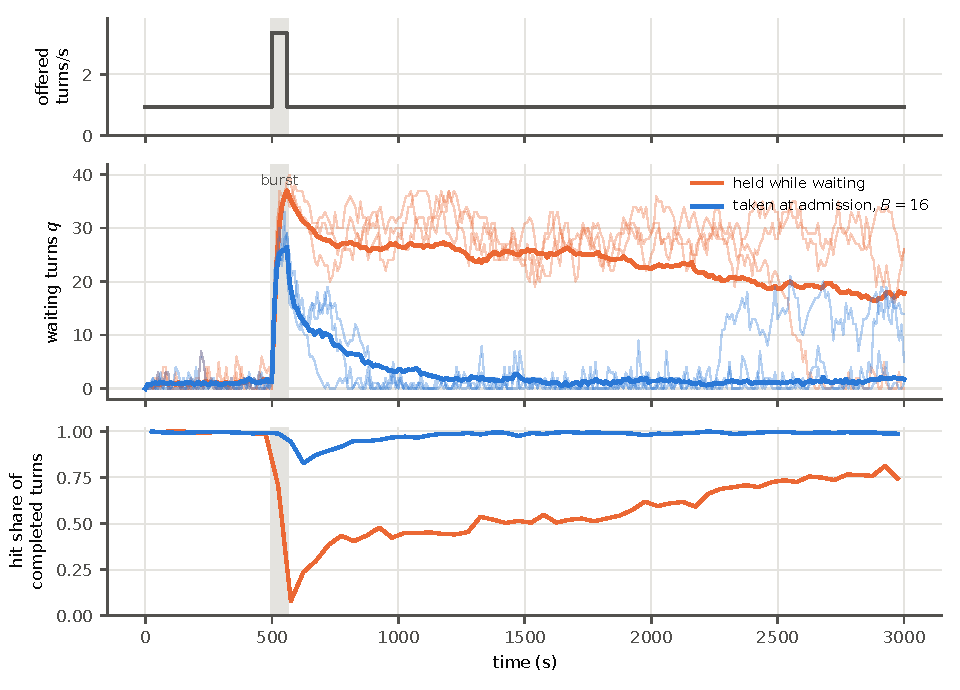
\includegraphics[width=\linewidth]{fig-meta-failure}
\caption{A metastable failure. Offered turn rate (top), waiting turns (middle: mean of
\metaFailPaths{} exact sample paths, three paths faint) and hit share of completed turns in
50\,s windows (bottom), for a queue-and-cache chain whose waiting turns hold memory and
for the same chain with memory taken at admission. $N=40$, $C=48$, memory
\metaFailA{} contexts per turn. The grey band is the burst.}\label{L7:fig:failure}
\end{figure}

\begin{figure}[h]\centering
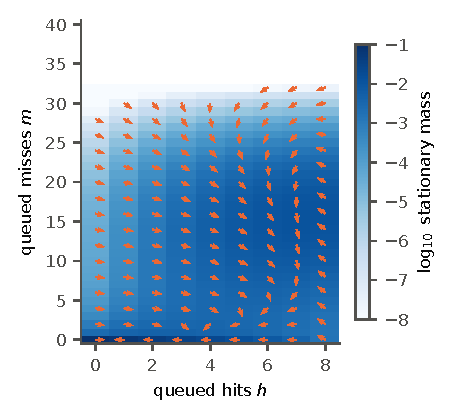
\includegraphics[width=0.48\linewidth]{fig-meta-drift}\hfill
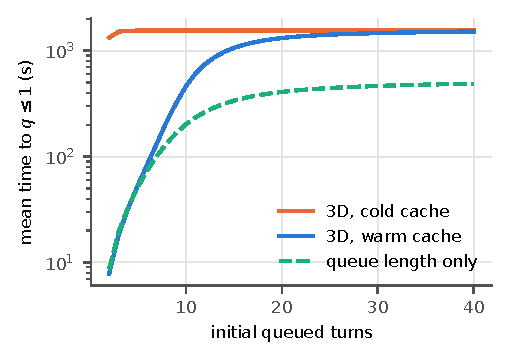
\includegraphics[width=0.48\linewidth]{fig-meta-recovery}
\caption{Queue-and-cache chain ($a=1$). Left: mean drift of the waiting hits and misses
(arrows, direction only) over the stationary mass. Right: mean time to $q\le1$ against the
initial queue, from waiting hits with a warm cache, from waiting misses after a flush, and
in the lumped chain.}\label{L7:fig:drift}
\end{figure}

\paragraph{Drift and recovery.} The mass sits at the empty queue and in a band of 16 to
32 waiting misses with at most \metaRecurrentH{} waiting hits (\cref{L7:fig:drift},
left). From ten waiting turns the recovery takes \metaRecWarmTen\,s with a warm cache and
\metaRecColdTen\,s after a flush, while the lumped chain predicts \metaRecLumpTen\,s; the
time rises steeply over the first ten to fifteen turns and then saturates (right).

\paragraph{Where metastability appears.} \Cref{L7:fig:region} maps the slowest relaxation
time over the memory $a$ held per waiting turn and the think time. The queue-length law
is bimodal only for $a\ge\metaBimodalAmin$, memory per waiting turn comparable to a
whole context, as \cref{L7:prop:hold} leads one to expect. An engine that allocates at
admission has a small $a$ for at most $B$ turns. One that holds a whole prompt's blocks
while the turn waits, as a disaggregated decoder does while it waits for a KV transfer,
has $a\approx1$ for every waiting turn.

\begin{figure}[h]\centering
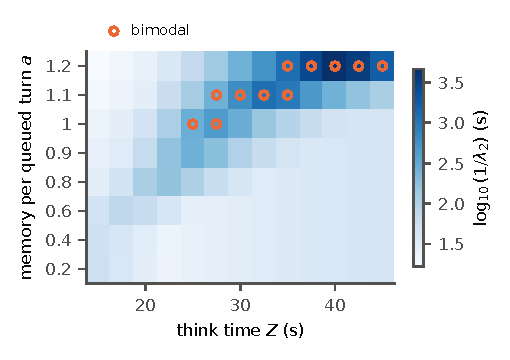
\includegraphics[width=0.58\linewidth]{fig-meta-region}
\caption{Queue-and-cache chain, $N=40$, $C=48$: $\log_{10}$ of the slowest relaxation
time; circles mark a bimodal queue-length law.}\label{L7:fig:region}
\end{figure}

\paragraph{vLLM's rules in serQ.} serQ's vLLM program allocates at admission, so the
prediction is a cliff without metastability (\cref{L7:fig:sweep}). From five seeds and a
cold or a warm start, the hit rate falls from \metaSqHitHigh{} at $Z=4$\,s to
\metaSqHitLow{} at $Z=1.5$\,s and the mean TTFT rises from \metaSqTtftHigh{} to
\metaSqTtftLow\,s; the two starts end within \metaSqColdWarmGap{} of each other at every
load, so there is no hysteresis. The cliff is \cref{L7:prop:rounds}(i): near saturation
the turns are served nearly round-robin and LRU evicts the next one in line. After a burst
at $Z=1.5$\,s the hit rate, \metaSqMinHit{} during the burst, is back within 0.05 of its
baseline \metaSqRecSixty\,s after a 60\,s burst and \metaSqRecThreeHundred\,s after a
300\,s burst (\cref{L7:fig:burst}b), against more than a thousand seconds in the chain
with $a=1$ (panel a).

\begin{figure}[h]\centering
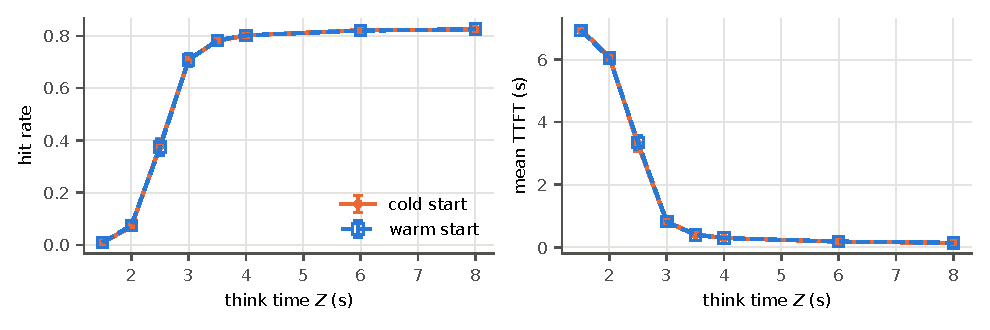
\includegraphics[width=\linewidth]{fig-meta-sweep}
\caption{serQ, vLLM's rules: hit rate and mean TTFT over 2000--4000\,s against the think
time, from a cold and a warm cache (five seeds, mean and standard deviation).}\label{L7:fig:sweep}
\end{figure}

\begin{figure}[h]\centering
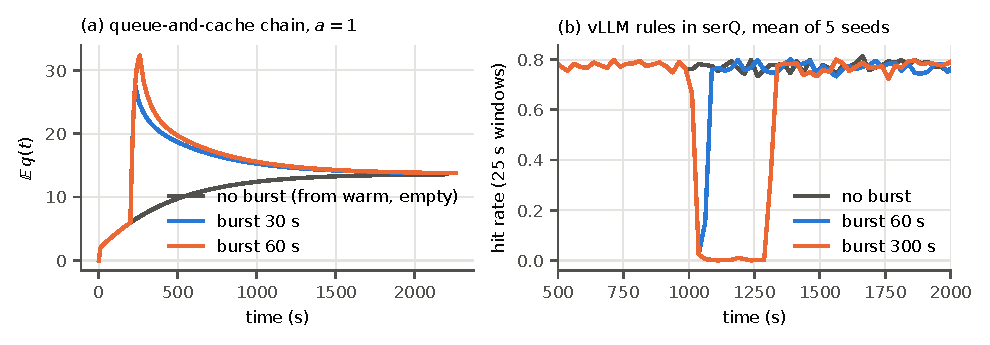
\includegraphics[width=\linewidth]{fig-meta-burst}
\caption{Bursts. (a) Queue-and-cache chain, $a=1$, think time 27\,s and 12\,s during the
burst, exact transient means. (b) serQ, think time 4\,s and 1.5\,s during the burst, hit
rate in 25\,s windows, mean of five seeds.}\label{L7:fig:burst}
\end{figure}

\paragraph{Calibration.} We fit a chain to serQ's hit-rate sweep and predict the bursts,
which the fit does not see. Service times come from serQ's engine utilisation, 0.037\,s
per hit and 0.336\,s per miss; memory is counted in contexts, $C\approx\metaAbC$, an
admitted turn adds $a=0.04$, and an admitted miss holds the prefix it recomputes. The
chain of \cref{L7:def:three} cannot be fitted (\cref{L7:fig:calibration}a): its best error
in hit rate is \metaPsRmse, and at the highest load it predicts \metaPsLowZ{} against
serQ's \metaSqLowZ. Under processor sharing a short hit overtakes the misses, so the hit
rate stays high under load. A chain that serves one turn at a time and evicts the next
turn in line, with a waiting prefix weighted $\beta$ against a thinking one, fits with
$C=\metaFifoC$, $\beta=\metaFifoBeta$ and an error of \metaFifoRmse. It predicts
recoveries of \metaPredRecSixty\,s after both held-out bursts, against serQ's
\metaSqRecSixtyB\,s and \metaSqRecThreeHundredB\,s (panel b). The order of service and the
identity of the LRU victim, the content of \cref{L7:prop:mattson,L7:prop:rounds}, are the
state a faithful model must keep.

\begin{figure}[h]\centering
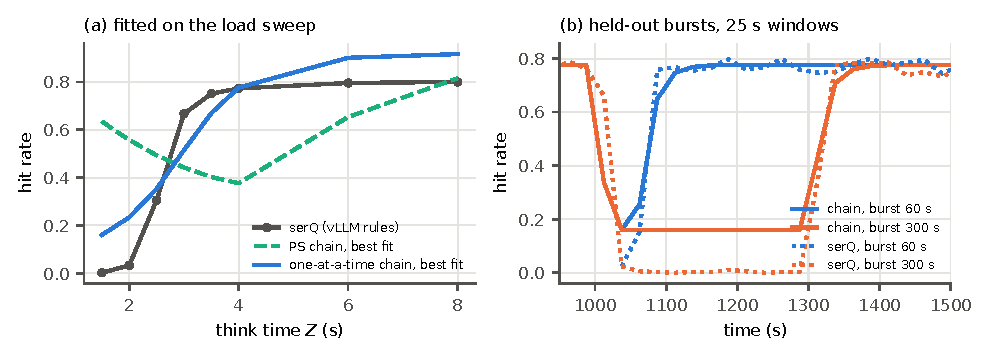
\includegraphics[width=\linewidth]{fig-meta-calibration}
\caption{Calibration against serQ. (a) Hit rate against the think time: serQ and the best
fits of the processor-sharing and the FCFS chains. (b) Held-out bursts.}\label{L7:fig:calibration}
\end{figure}

\section{Conclusions}\label{L7:sec:conclusions}

\begin{enumerate}
\item \emph{FCFS with LRU loses every prefix behind a queue of $C$.} A turn behind $C$
  others misses (\cref{L7:cor:behind}); under saturation LRU hits nothing, any rule at most
  $C$ of $N$ per round, and pinning $C$ sessions attains $C$ (\cref{L7:prop:rounds}). This
  is the cliff in serQ's run of vLLM's rules.
\item \emph{The stability limit is set by the miss work, the lifetime by the cache.} An
  FCFS--LRU replica is stable if and only if $\lambda S^{\mathrm{miss}}<1$, for every cache
  size; a larger cache lengthens the good state's lifetime exponentially in $C$ but does
  not move the limit (\cref{L7:thm:open}). Faster prefill or a cheaper restore moves it.
\item \emph{Take memory at admission.} Doing so never slows service or recovery, and it
  leaves no congested mode above the batch cap (\cref{L7:prop:hold}). After the same 60\,s
  burst, a replica whose waiting turns hold memory is still congested with probability
  \metaFailHeldEnd{} after 3000\,s; one that takes memory at admission has drained
  (\cref{L7:fig:failure}). Metastability
  appears when every waiting turn holds about a context of memory
  (\cref{L7:fig:region}), and serQ's admission-time engine shows a cliff without
  hysteresis (\cref{L7:fig:sweep}). Engines that reserve memory while a turn waits, such
  as a decoder waiting for a KV transfer, are the ones to test.
\item \emph{A predictive model must keep the waiting misses and the service order.}
  Queue length alone is exact for steady state and optimistic about recovery by a factor
  of about three (\cref{L7:sec:enough}); a processor-sharing chain cannot be calibrated to
  vLLM's rules, an FCFS chain can, and it predicts a recovery of \metaPredRecSixty\,s after held-out
  bursts where serQ shows \metaSqRecSixtyB{} and \metaSqRecThreeHundredB\,s.
\item \emph{Rank interventions by the question asked.} Steady state and recovery rank
  them differently (\cref{L7:tab:interventions}): the best response time comes from a
  faster prefill, the fastest recovery from more cache.
\end{enumerate}

\section{What is exact and what is approximate}\label{L7:sec:honest}

\begin{itemize}
\item \emph{Proved} (and checked in Lean, module \texttt{CacheOrder} and
  \texttt{Metastability}, except where noted): \cref{L7:prop:mattson,L7:prop:rounds},
  \cref{L7:cor:behind} (its FCFS step is in the proof above), \cref{L7:lem:bd} (its
  algebraic content; that $T_k$ and $R$ are hitting times is proved here only),
  \cref{L7:thm:open,L7:prop:hold}, and \cref{L7:lem:lump} (here only). Every chain number
  is computed from the generator, not simulated.
\item \emph{Simulation:} the serQ runs model vLLM's scheduler; they are not measurements
  of an engine.
\item \emph{Modelling choices:} prefixes of equal size and session-level LRU instead of
  blocks; the queue-length model of \cref{L7:thm:open}, in which the loss depends on the
  current queue rather than the queue a turn joined; exponential service; processor
  sharing or one turn at a time instead of a batched engine; no cost of pinned memory.
\item \emph{To be measured:} the loss onset, the slack $C-N$ and the memory per waiting
  turn on a real engine, with the burst protocol (normal load, a short burst, normal load;
  warm and flushed starts).
\end{itemize}

\section{Exercises}

\begin{exercise}\label{L7:ex:step}
Let $m(n)=\1\{n\ge C\}$ in the open queue, with $1/S^{\mathrm{miss}}<\lambda<1/S^{\mathrm{hit}}$.
Show that the fluid saddle is at $C$, and that the mean time to reach $C$ from the empty
queue is of order $(\lambda S^{\mathrm{hit}})^{-C}$.
\end{exercise}

\begin{exercise}\label{L7:ex:fifo}
In \cref{L7:prop:rounds}(i) let each round serve the $N$ sessions once, in an order
that may change from round to round. Show that LRU can then hit, and find the largest
number of hits in a round as a function of $N$ and $C$.
\end{exercise}

\begin{exercise}\label{L7:ex:cost}
Add a concurrency cost to \cref{L7:def:three}: pinned prefixes slow every turn by the
factor $1+\gamma\,\phi h/N$. Find, numerically, a $\gamma$ at which an interior $\phi$
minimises the recovery time.
\end{exercise}
